\documentclass[12pt]{article}
\usepackage[utf8]{inputenc}
\usepackage[spanish]{babel}
\decimalpoint
\usepackage{amsmath}
\usepackage{caption}
\usepackage{amsthm}
\usepackage{amssymb}
\usepackage{graphicx}
\usepackage[margin=0.9in]{geometry}
\usepackage{fancyhdr}
\usepackage[inline]{enumitem}
\usepackage{float}
\usepackage{cancel}
\usepackage{bigints}
\usepackage{color}
\usepackage{xcolor}
\usepackage{listingsutf8}
\usepackage{algorithm}
\usepackage{tocloft}
\usepackage[none]{hyphenat}
\usepackage{graphicx}
\usepackage{grffile}
\usepackage{tabularx}
\usepackage[nottoc,notlot,notlof]{tocbibind}
\usepackage{times}
\usepackage{color}
\definecolor{gray97}{gray}{.97}
\definecolor{gray75}{gray}{.75}
\definecolor{gray45}{gray}{.45}
\renewcommand{\cftsecleader}{\cftdotfill{\cftdotsep}}
\pagestyle{fancy}
\setlength{\headheight}{15pt} 
\lhead{Práctica 2 - Análisis temporal y notación de orden (Algoritmos de búsqueda)}
\rhead{\thepage}
\lfoot{ESCOM-IPN}
\renewcommand{\footrulewidth}{0.5pt}
\setlength{\parskip}{0.5em}
\newcommand{\ve}[1]{\overrightarrow{#1}}
\newcommand{\abs}[1]{\left\lvert #1 \right\lvert}
\date{26 de febrero de 2017}
\title{Pruebas a posteriori}
\author{Reporte 1}

\definecolor{pblue}{rgb}{0.13,0.13,1}
\definecolor{pgreen}{rgb}{0,0.5,0}
\definecolor{pred}{rgb}{0.9,0,0}
\definecolor{pgrey}{rgb}{0.46,0.45,0.48}
\lstset{tabsize=1}

\usepackage{listings}
\lstset{ frame=Ltb,
framerule=0pt,
aboveskip=0.5cm,
framextopmargin=3pt,
framexbottommargin=3pt,
framexleftmargin=0.4cm,
framesep=0pt,
rulesep=.4pt,
backgroundcolor=\color{gray97},
rulesepcolor=\color{black},
%
stringstyle=\ttfamily,
showstringspaces = false,
basicstyle=\small\ttfamily,
commentstyle=\color{gray45},
keywordstyle=\bfseries,
%
numbers=left,
numbersep=15pt,
numberstyle=\tiny,
numberfirstline = false,
breaklines=true,
}

% minimizar fragmentado de listados
\lstnewenvironment{listing}[1][]
{\lstset{#1}\pagebreak[0]}{\pagebreak[0]}

\lstdefinestyle{consola}
{basicstyle=\scriptsize\bf\ttfamily,
backgroundcolor=\color{gray75},
}

\lstdefinestyle{Java}
{language=Java,
}

%%%%%%%%%%%%%%%%%%%%%

\lstdefinestyle{customc}{
  belowcaptionskip=1\baselineskip,
  breaklines=true,
  frame=L,
  xleftmargin=\parindent,
  language=C,
  showstringspaces=false,
  basicstyle=\footnotesize\ttfamily,
  keywordstyle=\bfseries\color{green!40!black},
  commentstyle=\itshape\color{purple!40!black},
  identifierstyle=\color{blue},
  stringstyle=\color{orange},
}

\lstdefinestyle{customasm}{
  belowcaptionskip=1\baselineskip,
  frame=L,
  xleftmargin=\parindent,
  language=[x86masm]Assembler,
  basicstyle=\footnotesize\ttfamily,
  commentstyle=\itshape\color{purple!40!black},
}

\lstset{escapechar=@,style=customc}


    % =====  CODE EDITOR =========
    \lstdefinestyle{CompilandoStyle} {                              %This is Code Style
        backgroundcolor=\color{BlueGrey800MD},                      %Background Color  
        basicstyle=\tiny\color{white},                              %Font color
        commentstyle=\color{BlueGrey100MD},                         %Comment color
        stringstyle=\color{TealMD},                                 %String color
        keywordstyle=\color{Green100MD},                            %keywords color
        numberstyle=\tiny\color{TealMD},                            %Size of a number
        frame=shadowbox,                                            %Adds a frame around the code
        breakatwhitespace=true,                                     %Style                       
        breaklines=true,                                            %Style                   
        keepspaces=true,                                            %Style                   
        numbers=left,                                               %Style                   
        numbersep=10pt,                                             %Style 
        xleftmargin=\parindent,                                     %Style 
        tabsize=4                                                   %Style 
    }
 
    \lstset{style=CompilandoStyle}                                  %Use this style

    \usepackage{minted} % Paquete que permite citar codigo
    \usemintedstyle{borland} % Aqui se define el colorscheme para minted
    \setminted{
        fontsize = \scriptsize, % Ajusta el codigo a la hoja
        baselinestretch = 1,
        linenos, % set numbers
        breaklines=true, % Hace un salto de linea automatico en caso de que se llege al final de la line
        tabsize=3 
    }

%Permite crear columnas en el documento
\usepackage{multicol} 
\usepackage{color}
\usepackage{comment}
\newcommand{\tabitem}{~~\llap{\textbullet}~~}
\newcommand{\subtabitem}{~~~~\llap{\textbullet}~~}

\bibliographystyle{IEEEtran}
\begin{document}
		\begin{titlepage}
			\begin{center}
				
				% Upper part of the page. The '~' is needed because \\
				% only works if a paragraph has started.
				
				\noindent
				\begin{minipage}{0.5\textwidth}
					\begin{flushleft} \large
						\includegraphics[width=0.3\textwidth]{../ipn.png}
					\end{flushleft}
				\end{minipage}%
				\begin{minipage}{0.55\textwidth}
					\begin{flushright} \large
						\includegraphics[width=0.7\textwidth]{../escom.png}
					\end{flushright}
				\end{minipage}
				
				\textsc{\LARGE Instituto Politécnico Nacional}\\[0.5cm]
				
				\textsc{\Large Escuela Superior de Cómputo}\\[1cm]
				
				% Title
				
				{ \huge Práctica 2 - Análisis temporal y notación de orden (Algoritmos de búsqueda)\\[1cm] }
				
				{ \Large Unidad de aprendizaje: Análisis de Algoritmos} \\[1cm]
				
				{ \Large Grupo: 3CM3} \\[1cm]
				
				\noindent
				\begin{minipage}{0.5\textwidth}
					\begin{flushleft} \large
						\emph{Alumnos(a): "La naranja mecánica"}\\
						
						\begin{tabular}{ll}
					     Nicolás Sayago Abigail\\
					     Parra Garcilazo Cinthya Dolores\\
					     Ramos Díaz Enrique \\
					
					\end{tabular}
					\end{flushleft}
				\end{minipage}%
				\begin{minipage}{0.5\textwidth}
					\begin{flushright} \large
						\emph{Profesor(a): Edgardo Adrián Franco Martínez} \\
						  \\
					\end{flushright}
				\end{minipage}
				
					\begin{minipage}{0.5\textwidth}
					\begin{center} \large
						\includegraphics[width=0.8\textwidth]{../xd.jpg}
						\caption*{"La Naranja Mecánica"}
					\end{center}
				\end{minipage}

				\vfill
				
				% Bottom of the page
				{\large 3 de Octubre 2018}
			\end{center}
		\end{titlepage}
	
	\tableofcontents
	\newpage
	% /////////////////////////////////////////////////////////
	%			PLANTEAMIENTO DEL PROBLEMA
	% ////////////////////////////////////////////////////////
	\section{Planteamiento del problema}

	
	% /////////////////////////////////////////////////////////
	%			PLATAFORMA EXPERIMENTAL
	% ////////////////////////////////////////////////////////
    \section{Plataforma Experimental}
	
	    \textbf{Especificaciones de Hardware:}
	    \begin{itemize}
	        \item CPU: Intel Core-i5 6500 3.2 GHz
	        \item Memoria: RAM DDR4 5.9 GB 2133 MHz
	    \end{itemize}
    
	    \textbf{Compilador:} GCC version 7.3.0 desde la Terminal
	    
	    \textbf{Sistema Operativo:} Linux Ubuntu 18.04.1 LTS x64 

	% /////////////////////////////////////////////////////////
	%			ACTIVIDADES Y PRUEBAS
	% ////////////////////////////////////////////////////////
	
	\section{Actividades y Pruebas}
	
		% ----------------------------------------------------
		% 					BUSQUEDA LINEAL
		% ----------------------------------------------------
	    \subsection{Búsqueda Lineal}
	        \subsubsection{Análisis teórico a priori}
	        
	        \subsubsection{Ejecución del algoritmo}
            	\begin{figure}[H]
                	   \centering
                	   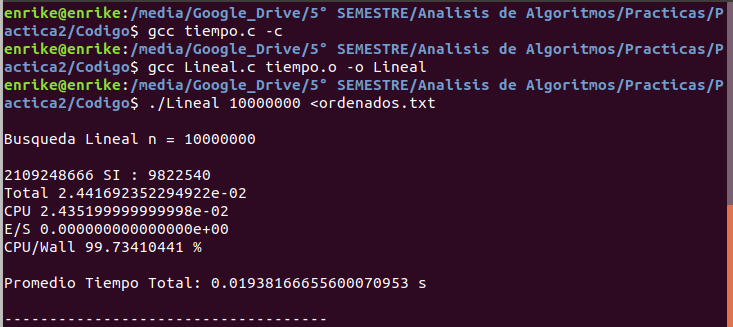
\includegraphics[width=0.8\textwidth]{images/pruebas/lineal.png}
                \end{figure}
	        
	        \subsubsection{Análisis temporal promedio}
            	\begin{figure}[H]
            	    \centering
                	   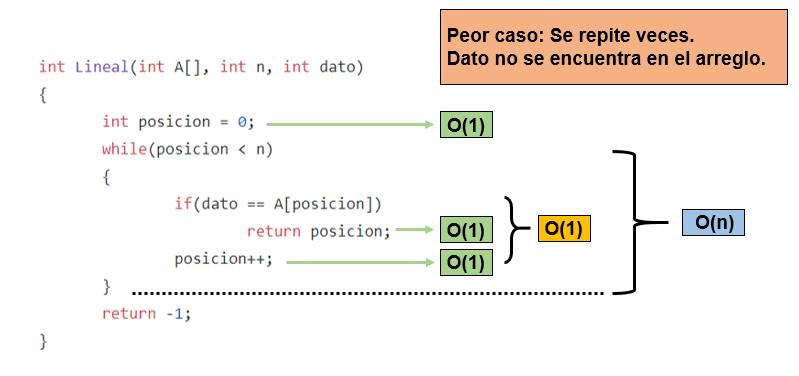
\includegraphics[width=0.8\textwidth]{images/tablas/Lineal.JPG}
                \end{figure}
        	
        	\subsubsection{Gráfica de comportamiento}
            	\begin{figure}[H]
            	    \centering
                	   \includegraphics[width=0.8\textwidth]{images/graficas/LinealGrafica.JPG}
                \end{figure}
    
        	\subsubsection{Aproximación Polinomial}
    
        	\subsubsection{Tiempo por cada operación básica}
    
        	\subsubsection{Evaluación de tamaños de problema n's}
    
    		\subsubsection{Cotas O mayúscula}
	
\newpage

		% ----------------------------------------------------
		% 					BUSQUEDA LINEAL HILOS
		% ----------------------------------------------------

		\subsection{Búsqueda Lineal (Hilos)}
			
			\subsubsection{Funcionamiento}
			
			\subsubsection{Ejecución del algoritmo}
				\begin{figure}[H]
			    	   \centering
			    	   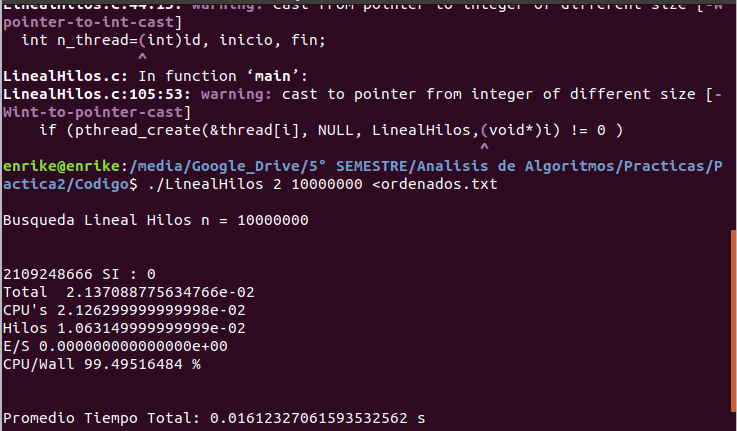
\includegraphics[width=0.8\textwidth]{images/pruebas/linealhilos.png}
			    \end{figure}
			
			\subsubsection{Análisis temporal promedio}
				\begin{figure}[H]
				    \centering
			    	   \includegraphics[width=0.8\textwidth]{images/tablas/LinealHilos.JPG}
			    \end{figure}
			
			\subsubsection{Gráfica de comportamiento}
				\begin{figure}[H]
				    \centering
			    	   \includegraphics[width=0.8\textwidth]{images/graficas/LinealHilosGrafica.JPG}
			    \end{figure}
			
			\subsubsection{Aproximación Polinomial}
			
			\subsubsection{Tiempo por cada operación básica}
			
			\subsubsection{Evaluación de tamaños de problema n's}
			
			\subsubsection{Cotas O mayúscula}
			
\newpage

		% ----------------------------------------------------
		% 					BUSQUEDA BINARIA
		% ----------------------------------------------------	
	
		\subsection{Búsqueda Binaria}
			
			\subsubsection{Análisis teórico a priori}
			
			\subsubsection{Ejecución del algoritmo}
				\begin{figure}[H]
			    	   \centering
			    	   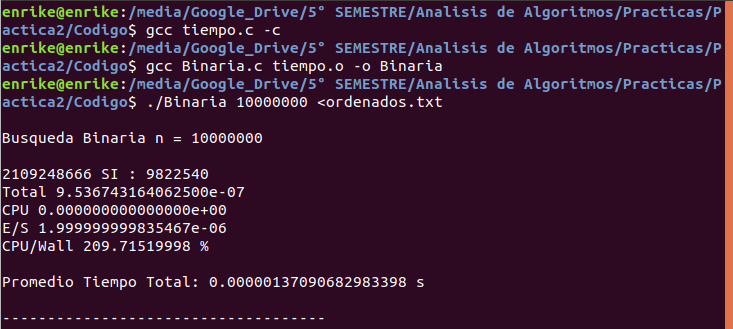
\includegraphics[width=0.8\textwidth]{images/pruebas/binaria.png}
			    \end{figure}
			
			\subsubsection{Análisis temporal promedio}
				\begin{figure}[H]
			    	   \centering
			    	   \includegraphics[scale=0.75]{images/tablas/binaria.PNG}
			    \end{figure}
			
			\subsubsection{Gráfica de comportamiento}
				\begin{figure}[H]
			    	   \centering
			    	   \includegraphics[scale=0.8]{images/graficas/binaria.PNG}
			    \end{figure}
			
			\subsubsection{Aproximación Polinomial}
				\begin{figure}[H]
			    	   \centering
			    	   \includegraphics[width=0.75\textwidth]{images/polinomios/binaria.PNG}
			    	   \caption*{\textbf{Grado 5: $7.20374\times10^{-7} + 2.42704\times10^{-13} x - 6.58073\times10^{-20} x^2 + 
			            1.16759\times10^{-26} x^3 - 1.10283\times10^{-33} x^4 + 4.15462\times10^{-41} x^5$}}
			    \end{figure}
			
			\subsubsection{Tiempo por cada operación básica}
			
			\subsubsection{Evaluación de tamaños de problema n's}
			
			\subsubsection{Cotas O mayúscula}
				
\newpage
		% ----------------------------------------------------
		% 					BUSQUEDA BINARIA HILOS
		% ----------------------------------------------------

		\subsection{Búsqueda Binaria (Hilos)}
			
			\subsubsection{Funcionamiento}
			
			\subsubsection{Ejecución del algoritmo}
				\begin{figure}[H]
			    	   \centering
			    	   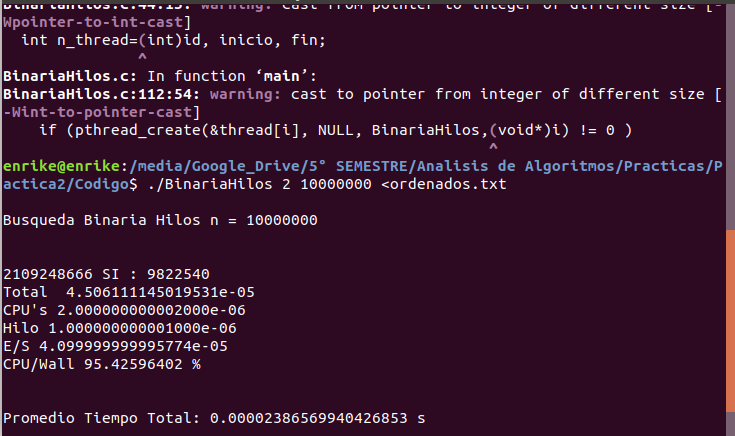
\includegraphics[width=0.8\textwidth]{images/pruebas/binariahilos.png}
			    \end{figure}
			
			\subsubsection{Análisis temporal promedio}
				\begin{figure}[H]
			    	   \centering
			    	   \includegraphics[scale=0.75]{images/tablas/binariahilos.PNG}
			    \end{figure}
			
			\subsubsection{Gráfica de comportamiento}
				\begin{figure}[H]
			    	   \centering
			    	   \includegraphics[scale=0.8]{images/graficas/binariahilos.PNG}
			    \end{figure}
			
			\subsubsection{Aproximación Polinomial}
				\begin{figure}[H]
			    	   \centering
			    	   \includegraphics[width=0.75\textwidth]{images/polinomios/binariahilos.PNG}
			    	   \caption*{\textbf{Grado 8: $0.0000208055 + 1.3099\times10^{-11} x - 2.07682\times10^{-17} x^2 + 1.34802\times10^-{23} x^3 - 4.71663\times10^-30 x^4 + 9.64\times10^{-37} x^5 - 1.13965\times10^{-43} x^6 + 7.15912\times10^{-51} x^7 - 1.83887\times10^{-58} x^8$}}
			    \end{figure}
			
			\subsubsection{Tiempo por cada operación básica}
			
			\subsubsection{Evaluación de tamaños de problema n's}
			
			\subsubsection{Cotas O mayúscula}
		
\newpage

		% ----------------------------------------------------
		% 				ARBOL DE BUSQUEDA BINARIA
		% ----------------------------------------------------

		\subsection{Árbol de Búsqueda Binaria}
			
			\subsubsection{Análisis teórico a priori}
			
			\subsubsection{¿Por qué no usar hilos?}
			
			\subsubsection{Ejecución del algoritmo}
				\begin{figure}[H]
			    	   \centering
			    	   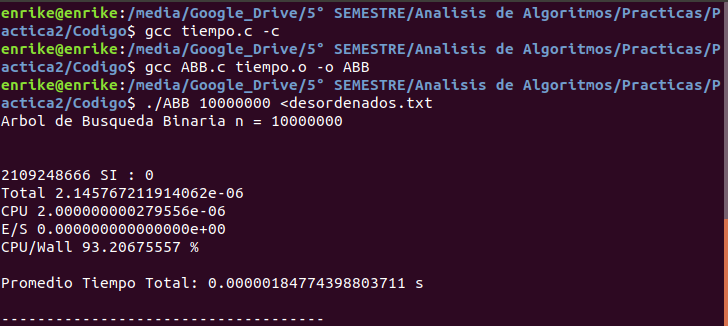
\includegraphics[width=0.8\textwidth]{images/pruebas/abb.png}
			    \end{figure}

			\subsubsection{Análisis temporal promedio}
				\begin{figure}[H]
			    	   \centering
			    	   \includegraphics[scale=0.75]{images/tablas/ABB.PNG}
			    \end{figure}
			
			\subsubsection{Gráfica de comportamiento}
				\begin{figure}[H]
			    	   \centering
			    	   \includegraphics[scale=0.8]{images/graficas/ABB.PNG}
			    \end{figure}
			
			\subsubsection{Aproximación Polinomial}
			
			\subsubsection{Tiempo por cada operación básica}
			
			\subsubsection{Evaluación de tamaños de problema n's}
			
			\subsubsection{Cotas O mayúscula}
			
			\subsection{Comparativa gráfica de comportamiento (Tiempo Real promedio)}
			
			\subsection{Comparativa de aproximaciones polinomiales}

		% ----------------------------------------------------
		% 					CUESTIONARIO
		% ----------------------------------------------------

		\subsection{Cuestionario}
		\begin{enumerate}
			        \item ¿Cuál de los 3 algoritmos es más fácil de implementar?\\
			        .\\
			        
			        \item ¿Cuál de los 3 algoritmos es más difícil de implementar?\\
			        .\\
			        
			        \item ¿Cuál de los 3 algoritmos es el más difícil de implementar en su variante con hilos?\\
			        .\\
			        
			        \item ¿Cuál de los 3 algoritmos en su variante con hilos resultó ser más rápido?\\
			        .\\
			        
			        \item ¿Cuál algoritmo tiene menor complejidad temporal?\\
	                .\\
			        
			        \item ¿Cuál algoritmo tiene mayor complejidad temporal?\\
			        . \\
			        
			        
			        \item ¿El comportamiento experimental de los algoritmos era el esperado?¿Por qué?\\
			        .\\
			        
			        \item ¿Sus resultados experimentales difieren mucho de los análisis teóricos que se analizaron? ¿A que se debe?\\
			        .\\
			        
			        \item ¿Los resultados experimentales de las implementaciones con hilos de los algoritmos realmente tardaron F(t)/#hilos de su implementación sin hilos?\\
			        .\\
			        
			        \item ¿Cuál es el \% de mejora que tiene cada uno de los algoritmos en su variante con hilos?¿Es lo que esperabas?¿Por qué?\\
			        .\\
			        
			        \item ¿Existió un entorno controlado para realizar las pruebas experimentales?¿Cuál fue?
			        .\\
			        
			        \item ¿Si solo se realizara el análisis teórico de un algoritmo antes de implementarlo, podrías asegurar cuál es el mejor?\\
			        .\\
			        
			        \item ¿Qué tan difícil fue realizar el análisis teórico de cada algoritmo?\\
			        .\\
			        
			        \item ¿Qué recomendaciones darían a nuevos equipos para realizar esta práctica?\\
			        .\\
			        
			    \end{enumerate}
	
	% /////////////////////////////////////////////////////////
	%					ERRORES DETECTADOS
	% ////////////////////////////////////////////////////////
	
	\section{Errores detectados}

\newpage

	% /////////////////////////////////////////////////////////
	%							ANEXOS
	% ////////////////////////////////////////////////////////

	\section{Anexos}

		\subsection{Búsqueda Lineal}
		    \inputminted{c++}{Code/Lineal.c}
		 
		 \subsection{Búsqueda Lineal (Hilos)}
		    \inputminted{c++}{Code/LinealHilos.c}
		    
		 \subsection{Búsqueda Binaria}
		    \inputminted{c++}{Code/Binaria.c}
		 
		 \subsection{Búsqueda Binaria (Hilos)}
		    \inputminted{c++}{Code/BinariaHilos.c}
		 
		 \subsection{Arbin.h}
		    \inputminted{c++}{Code/Arbin.h}
		 
		 \subsection{Árbol de Búsqueda Binaria}
		    \inputminted{c++}{Code/ABB.c}
		 
		 \subsection{Script de Compilación}
		 \inputminted{c++}{Code/script.c}

	% /////////////////////////////////////////////////////////
	%						BIBLIOGRAFIA
	% ////////////////////////////////////////////////////////
	
	\section{Bibliografía}
	
	$[1]$ E. A. Franco Martínez, “Análisis temporal y notación de orden (Algoritmos de búsqueda)” Análisis de Algoritmos, Escuela Superior de Computación, Instituto Politécnico Nacional,
    Ciudad de México, México, Practica01.pdf, Sep. 2018
  
    $[2]$ (2018) WolframAlpha. Accessed september 2018. [Online]. \\Available: http://www.wolframalpha.com/

	\nocite{ref2}
	\bibliography{referencias}
     
\end{document}